\documentclass[12pt]{article}

%paquetes del idioma y codificacion
\usepackage[spanish]{babel}
\usepackage[utf8]{inputenc}
\usepackage[T1]{fontenc}
\usepackage{bookman}

%el indice
\usepackage{makeidx}

%paquetes matematicos
\usepackage{amsmath, amsfonts, amssymb}

%dimensiones
\usepackage[left=2.5cm, right=2.5cm, top=3cm]{geometry}

%para escribir codigo
\usepackage{listings}

% para contraer referencias
\usepackage{cite}

%para las imagenes y mas...
\usepackage{graphicx}
\usepackage{subfig}
\graphicspath{ {imagenes/} }
\usepackage{float}


\title{Segundo Entrega de Programas}
\author{Eslí Joana Osorio Rodríguez}


\begin{document}


\maketitle

\newpage

\tableofcontents

\newpage

\section{Autómata No Determinista}
Se desea realizar un programa el cual se un autómata no determinista que verificara si una cadena acaba en 01 y si es así la cadena será válida. La evaluación del estado tendrá que ser de forma dinámica y con varios estados ya que un solo carácter entrante nos podrá llevar a dos estados o hará que un estado truene mientras que otro abre.
 \cite{automatas}

\subsection{Código fuente}
El programa para está problema fue escrito en el lenguaje Python\\

Archivo: afn.py
\lstset{language=C, breaklines=true, basicstyle=\footnotesize}
\begin{lstlisting}[frame=single]
from random import *
def menu():
	entra=1
	while entra==1:
		print("\t\tSeleccione la opcion deseada\n 1.-Manual\n2.-Automatico\n")
		opc=str(input())
		print(opc)
		if opc=='1':
			manual()
		elif opc=='2':
			automatico()
		print("desea regresar?\n1.-Si\,2.-No\n")
		entra=int(input())
	print ("\t\tADIOS\n")

def manual():
	print("Ingresa un numero\n")
	numero=input()
	if(automata(numero)==1):
		print("Valida")
	else:
		("No Valida")

def automatico():
	n=""
	l=randint(1,1000)
	x=0
	while(x<l):
	    n+=choice(['0', '1'])
	    x += 1
	if(automata(n)==1):
		print("Valida")
	else:
		print("No Valida")

def automata(cadena):
	caminos = []
	caminos.append(['0'])
	for caracter in cadena:
		if(caracter=='0'):
			auxiliar=caminos[-1][:]
			while('2' in auxiliar):
				auxiliar.insert(auxiliar.index('2'),'x')
				auxiliar.pop(auxiliar.index('2'))
			while('1' in auxiliar):
				auxiliar.insert(auxiliar.index('1'),'x')
				auxiliar.pop(auxiliar.index('1'))
			auxiliar.append('1')
			caminos.append(auxiliar)
		elif(caracter=='1'):
			auxiliar=caminos[-1][:]
			while('2' in auxiliar):
				auxiliar.insert(auxiliar.index('2'),'x')
				auxiliar.pop(auxiliar.index('2'))
			while('1' in auxiliar):
				auxiliar.insert(auxiliar.index('1'),'2')
				auxiliar.pop(auxiliar.index('1'))
			caminos.append(auxiliar)
		else:
			return 0
	rellenarMatriz(caminos)
	for i in caminos:
		print(i)
	if(caminos[-1][-1]=='2'):
		caminos=[]
		return 1
	else:
		caminos=[]
		return 2

def rellenarMatriz(matriz):
	e=0
	while(e<len(matriz)):
		i=len(matriz[e])
		while(i<len(matriz[-1])-1):
			matriz[e].append(' x')
			i+=1
		e+=1
	e=0
	while(e<len(matriz) and len(matriz[e])!=len(matriz[-1])):
		matriz[e].append(matriz[e][0])
		e+=1
menu()
\end{lstlisting}

\subsection{Pruebas}
En cuanto a las pruebas, a continuación se mostraran una serie de imágenes capturadas al momento de ejecutar el programa. Los resultados arrojados por el programa anterior son:

Modo manual:

\begin{figure}[H]
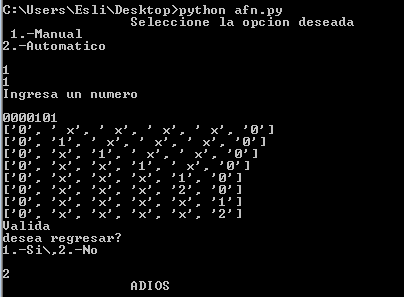
\includegraphics[width=\textwidth, height=9cm]{manual_afn}
\label{fig:manual_afn}
\caption{Ejecucion manual con cadena 0000101}
\end{figure}

Modo automatico:

\begin{figure}[H]
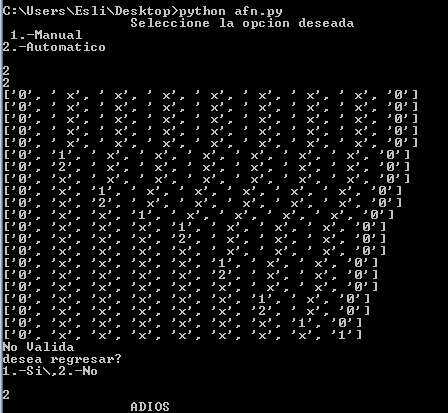
\includegraphics[width=\textwidth, height=11cm]{auto_afn}
\label{fig:manual_afn}
\caption{Ejecucion con cadena generada automaticamente }
\end{figure}

\newpage
\section{WEB/EBAY}
En este autómata se realizara una nueva modalidad del autómata buscador de texto como en el primer parcial que se busca las cadenas de terminación en ere, solo que este autómata reconocerá las cadenas que incluyen web o ebay entonces es como un nuevo modo del mismo autómata.
\subsection{Código fuente}
El programa para está problema fue escrito en el lenguaje Python\\

Archivo: web.py
\lstset{language=C, breaklines=true, basicstyle=\footnotesize}
\begin{lstlisting}[frame=single]
def grafico():
	root = 	Tk()
	root.title('Grafico')
	p=Canvas(root,width=1000,height=700)
	p.pack()
	p.create_line(140,325,250,200)
	p.create_line(140,375,250,500)
	p.create_line(350,200,650,200)
	p.create_line(350,500,850,500)
	p.create_line(100,10,100,690)
	p.create_line(700,10,700,690)
	p.create_line(100,10,700,10)
	p.create_line(100,690,900,690)
	p.create_line(100,50,500,50)
	p.create_line(100,100,300,100)
	p.create_line(320,100,670,100)
	p.create_line(300,100,300,650)
	p.create_line(320,100,320,200)
	p.create_line(100,650,300,650)
	p.create_line(500,50,500,150)
	p.create_line(500,550,500,700)
	p.create_line(100,675,500,675)
	p.create_line(470,100,470,200)
	p.create_line(670,100,670,300)
	p.create_line(900,690,900,350)
	p.create_line(880,640,880,530)
	p.create_line(330,640,330,530)
	p.create_line(530,640,530,350)
	p.create_line(730,640,730,350)
	p.create_line(330,640,880,640)
	p.create_line(300,350,900,350)
	p.create_line(320,300,670,300)
	p.create_line(320,300,320,500)
	p.create_line(520,180,520,300)
	p.create_oval(50, 300, 150, 400,fill="pink")
	p.create_oval(250, 150, 350, 250,fill="pink")
	p.create_oval(450, 150, 550, 250,fill="pink")
	p.create_oval(650, 150, 750, 250,fill="pink")
	p.create_oval(250, 450, 350, 550,fill="pink")
	p.create_oval(450, 450, 550, 550,fill="pink")
	p.create_oval(650, 450, 750, 550,fill="pink")
	p.create_oval(850, 450, 950, 550,fill="pink")
	p.create_oval(95, 95, 105, 105,fill="black")
	p.create_oval(95, 45, 105, 55,fill="black")
	p.create_oval(95, 5, 105, 15,fill="black")
	p.create_oval(95, 290, 105, 300,fill="black")
	p.create_oval(95, 400, 105, 410,fill="black")
	p.create_oval(95, 645, 105, 655,fill="black")
	p.create_oval(95, 670, 105, 680,fill="black")
	p.create_oval(95, 685, 105, 695,fill="black")
	p.create_oval(695, 685, 705, 695,fill="black")
	p.create_oval(725, 645, 735, 635,fill="black")
	p.create_oval(725, 355, 735, 345,fill="black")
	p.create_oval(525, 645, 535, 635,fill="black")
	p.create_oval(525, 355, 535, 345,fill="black")
	p.create_oval(325, 550, 335, 540,fill="black")
	p.create_oval(295, 355, 305, 345,fill="black")
	p.create_oval(295, 260, 305, 250,fill="black")
	p.create_oval(315, 155, 325, 145,fill="black")
	p.create_oval(475, 95, 465, 105,fill="black")
	p.create_oval(675, 95, 665, 105,fill="black")
	p.create_oval(440, 195, 450, 205,fill="black")
	p.create_oval(640, 195, 650, 205,fill="black")
	p.create_oval(240, 195, 250, 205,fill="black")
	p.create_oval(440, 495, 450, 505,fill="black")
	p.create_oval(640, 495, 650, 505,fill="black")
	p.create_oval(240, 495, 250, 505,fill="black")
	p.create_oval(840, 495, 850, 505,fill="black")
	p.create_oval(515, 305, 525, 295,fill="black")
	p.create_oval(315, 455, 325, 445,fill="black")
	l=Label(root,text="w")
	l.place(x=200,y=260)
	l=Label(root,text="e")
	l.place(x=400,y=180)
	l=Label(root,text="b")
	l.place(x=600,y=180)
	l=Label(root,text="y")
	l.place(x=800,y=480)
	l=Label(root,text="a")
	l.place(x=600,y=480)
	l=Label(root,text="b")
	l.place(x=400,y=480)
	l=Label(root,text="e")
	l.place(x=200,y=420)
	l=Label(root,text="w")
	l.place(x=300,y=300)
	l=Label(root,text="w")
	l.place(x=400,y=340)
	l=Label(root,text="w")
	l.place(x=600,y=340)
	l=Label(root,text="w")
	l.place(x=800,y=340)
	l=Label(root,text="e")
	l.place(x=400,y=640)
	l=Label(root,text="e")
	l.place(x=600,y=640)
	l=Label(root,text="e")
	l.place(x=800,y=640)
	l=Label(root,text="w")
	l.place(x=400,y=100)
	l=Label(root,text="w")
	l.place(x=600,y=100)
	l=Label(root,text="-a-e-w")
	l.place(x=600,y=15)
	l=Label(root,text="-b-e-w")
	l.place(x=400,y=30)
	l=Label(root,text="-e-w")
	l.place(x=200,y=90)
	l=Label(root,text="-b-e-w")
	l.place(x=200,y=620)
	l=Label(root,text="-a-e-w")
	l.place(x=400,y=665)
	l=Label(root,text="-a-y-w")
	l.place(x=600,y=675)
	l=Label(root,text="-e-w")
	l.place(x=800,y=675)
	l=Label(root,text="e")
	l.place(x=420,y=290)
	l=Label(root,text="e")
	l.place(x=620,y=290)
	l=Label(root,text="q0",bg="pink")
	l.place(x=90,y=330)
	l=Label(root,text="q1",bg="pink")
	l.place(x=290,y=180)
	l=Label(root,text="q2",bg="pink")
	l.place(x=490,y=180)
	l=Label(root,text="q3",bg="pink")
	l.place(x=690,y=180)
	l=Label(root,text="q4",bg="pink")
	l.place(x=290,y=480)
	l=Label(root,text="q5",bg="pink")
	l.place(x=490,y=480)
	l=Label(root,text="q6",bg="pink")
	l.place(x=690,y=480)
	l=Label(root,text="q7",bg="pink")
	l.place(x=890,y=480)
	l=Label(root,text="w")
	l.pack()
	l.place(x=0,y=0)
	root.mainloop()

def manual():
		cadena=""
		ubi=open ("Camino.txt","w")
		ubi.close()
		Coordenadas=open ("Coordenadas.txt","w")
		Coordenadas.close()
		print ("\t Usted eligio el modo manual\n Ingrese el texto porfavor")
		cadena=input ()
		archivo=open ("Manual.txt","w")
		archivo.write(cadena)
		archivo.close()
		fp=open ("Validado.txt","w")
		fp.close()
		revision(1)
def automatico():
		cadena =""
		ubi=open ("Camino.txt","w")
		ubi.close()
		Coordenadas=open ("Coordenadas.txt","w")
		Coordenadas.close()
		print ("\t Usted eligio el modo automatico")
		archivo=open ("Automatico.txt","r")
		archivo.read()
		archivo.close()
		fp=open ("Validado.txt","w")
		fp.close()
		revision(2)
def revision(j):
		if j==1:
			archivo= open("Manual.txt","r")
		elif j==2:
			archivo= open("Automatico.txt","r")
		y=0
		for linea in archivo:
			cadena=linea
			estados(cadena, y)
			y=y+1
		archivo.close()
		
		
def estados(cadena, y):
	ubi=open ("Camino.txt","a")
	Coordenadas=open ("Coordenadas.txt","a")
	caracter=0
	x=0
	palabra=cadena.split()
	ban2=0
	ban1=0
	for i in palabra:
		ban1=0
		ban2=0
		tamano=len(i)
		estado=0
		c=0
		for a in (i+","):		
			if estado==0:
				ubi.write("q0 -"+a+"-->")
				if a=="e" or a=="E":
					estado=4
				elif a=="w" or a=="W":
					estado=1
				else :
					estado=0	
			elif estado==1:
				ubi.write("q1 -"+a+"-->")
				if a=="e" or a=="E":
					estado=2
				elif a=="w" or a=="W":
					estado=1
				else:
					estado=0
			elif estado==2:
				ubi.write("q2 -"+a+"-->")
				if a=="e" or a=="E":
					estado=4
				elif a=="b" or a=="B":
					estado=3
				else :
					estado=0
			elif estado==3:
				guardar(i)
				ubi.write("q3-"+a+"-->FIN Valida\n")
				ban1=1
				if a=="a" or a=="A":
					estado=6
				elif a=="w" or a=="W":
					estao=1
				elif a=="e" or a =="E":
					estado=4
				else:
					estado=0
			elif estado==4:
				ubi.write("q4 --->")
				if a=="e" or a=="E":
					estado=4
				elif a=="w" or a=="W":
					estado=1
				elif a=="b" or a=="B":
					estado=5
				else:
					estado=0
			elif estado==5:
				ubi.write("q5 -"+a+"-->")
				if a=="e" or a=="E":
					estado=4
				elif a=="w" or a=="W":
					estado=1
				elif a=="a" or a=="A":
					estado=6
				else:
					estado=0
			elif estado==6:
				ubi.write("q6 -"+a+"-->")
				if a=="e" or a=="E":
					estado=4
				elif a=="w" or a=="W":
					estado=1
				elif a=="y" or a=="Y":
					estado=7
				else:
					estado=0
			elif estado==7:
				ubi.write("q7 --->FIN Valida\n")
				if a=="e" or a=="E":
					estado=4
				elif a=="w" or a=="W":
					estado=1
				else:
					estado=0
				if ban1==0:
					guardar (i)
					ban1=1
			
		x=x+1
		if ban1==1:
			Coordenadas.write("Ubicacion:" + str(y+1) + "," + str(x) +  "\n")	
		elif ban1==0:
			ubi.write("No Valida\n")
				
def guardar(i):
	palabra=i
	valida=open ("Validado.txt","a")
	valida.write(palabra)
	valida.write("\n")
	valida.close()
def menu():
	entra=1
	while entra==1:
		print("\t\tSeleccione la opcion deseada\n 1.-Manual\n2.-Automatico\n3.-Grafico\n")
		opc=str(input())
		#opc=str(random.randrange(1,4))
		if opc=='1':
			manual()
		elif opc=='2':
			automatico()
		elif opc=='3':
			print("\t\tFue seleccionado el modo Grafico\n")
			grafico()
		print("desea regresar?\n1.-Si\,2.-No\n")
		entra=int(input())
		#entra=random.randrange(0,2)
	print ("\t\tADIOS\n")

menu()

\end{lstlisting}

\subsection{Pruebas}
En cuanto a las pruebas, a continuación se mostraran una serie de imágenes capturadas al momento de ejecutar el programa. Los resultados arrojados por el programa anterior son:

Modo manual:

\begin{figure}[H]
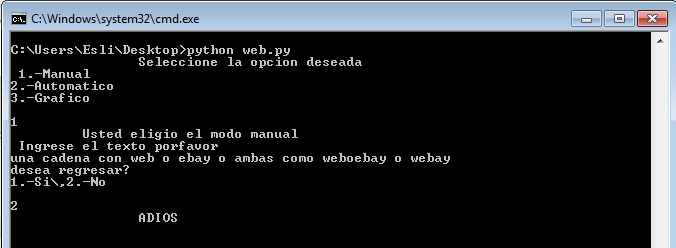
\includegraphics[width=\textwidth, height=9cm]{manual_web}
\label{fig:manual_afn}
\caption{Ejecucion manual con cadena 0000101}
\end{figure}

Modo automatico:

\begin{figure}[H]
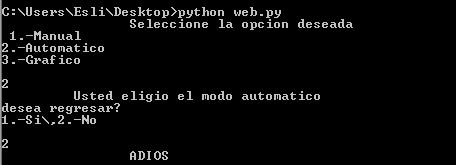
\includegraphics[width=15cm, height=7cm]{auto_web}
\label{fig:manual_afn}
\caption{Ejecucion con cadenas en un archivo }
\end{figure}

\begin{figure}[H]
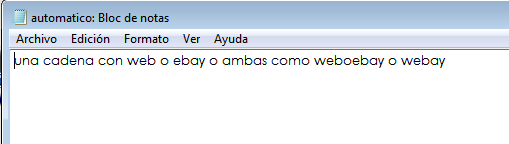
\includegraphics[width=15cm, height=7cm]{auto_web_archivo}
\label{fig:manual_afn}
\caption{El archivo para el modo automatico}
\end{figure}

Para ambos casos la salida para los archivos de caminos y valido fueron las siguientes:

\begin{figure}[H]
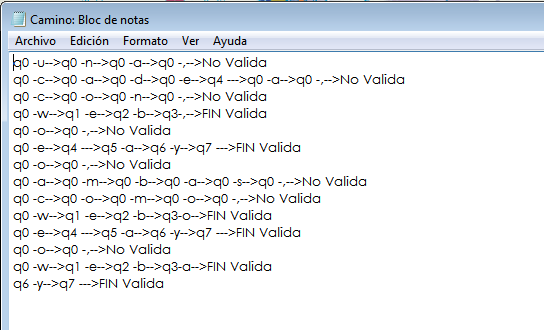
\includegraphics[width=\textwidth, height=15cm]{web_caminos}
\label{fig:manual_afn}
\caption{Caminos.txt}
\end{figure}

\begin{figure}[H]
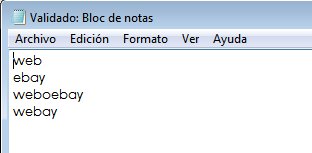
\includegraphics[width=15cm, height=5cm]{web_validos}
\label{fig:manual_afn}
\caption{Validos.txt}
\end{figure}

\newpage
\section{Planetas}
En este autómata se realizara una nueva modalidad del autómata buscador de texto como en el primer parcial que se busca las cadenas de El programa generara todas las combinaciones que se le asignen a un número determinado repartido en 3 especies ya que este es el chiste del programa. De inicio las combinaciones en las cuales una de las especies es la dominante se descartara y solo se trabajara con las combinaciones que requieren un proceso para saber si pueden llegar a terminar.
\subsection{Código fuente}
El programa para está problema fue escrito en el lenguaje Python\\

Archivo: planetas.py
\lstset{language=C, breaklines=true, basicstyle=\footnotesize}
\begin{lstlisting}[frame=single]
from random import *
def combinar(combinaciones,n):
	for x in range(0,n+1):  
		for y in range(0,n+1):
			for z in range(0,n+1):
				if((x+y+z)==n):
					if( (x!=0 and y!=0) or (x!=0 and z!=0) or (z!=0 and y!=0) ):
						combinaciones.append([x,y,z])
	return combinaciones

def listaFinal(combinacion):
	if(combinacion[0]==0 and combinacion[1]==0):
		return 1
	elif(combinacion[0]==0 and combinacion[2]==0):
		return 1
	elif(combinacion[2]==0 and combinacion[1]==0):
		return 1
	else:
		return 0

def repetido(combinacion,historial):
	if(historial==[]):
		return 0
	for casilla in historial:
		if(casilla==combinacion):
			return 1
	return 0

def automata(especies,historial):
	combinacion=especies.copy()
	r=repetido(combinacion.copy(),historial.copy())
	final=listaFinal(combinacion.copy())
	file1=open("No_fallan.txt","a")
	file2=open("Fallan.txt","a")
	if(r==1):
		historial.append(especies.copy())
		file1.write(str(historial)+" No Falla \n")
	elif(final==1):
		historial.append(especies.copy())
		file2.write(str(historial)+" Falla \n")
	else:
		historial.append(combinacion.copy())
		if(combinacion[0]==0):
			combinacion[0]+=2
			combinacion[1]-=1
			combinacion[2]-=1
			automata(combinacion.copy(),historial.copy())
		elif(combinacion[1]==0):
			combinacion[1]+=2
			combinacion[0]-=1
			combinacion[2]-=1
			automata(combinacion.copy(),historial.copy())
		elif(combinacion[2]==0):
			combinacion[2]+=2
			combinacion[1]-=1
			combinacion[0]-=1
			automata(combinacion.copy(),historial.copy())
		else:
			proceso1=combinacion.copy()
			proceso1[2]+=2
			proceso1[1]-=1
			proceso1[0]-=1
			proceso2=combinacion.copy()
			proceso2[1]+=2
			proceso2[0]-=1
			proceso2[2]-=1
			proceso3=combinacion.copy()
			proceso3[0]+=2
			proceso3[1]-=1
			proceso3[2]-=1
			automata(proceso1.copy(),historial.copy())
			automata(proceso2.copy(),historial.copy())
			automata(proceso3.copy(),historial.copy())
	file1.close()
	file2.close()

def menu():
	file1=open("Fallan.txt","w")
	file2=open("No_fallan.txt","w")
	file1.close()
	file2.close()
	entra=1
	while entra==1:
		print("\t\tSeleccione la opcion deseada\n 1.-Manual\n2.-Automatico\n")
		opc=str(input())
		print(opc)
		if opc=='1':
			manual()
		elif opc=='2':
			automatico()
		print("desea regresar?\n1.-Si\,2.-No\n")
		entra=int(input())
	print ("\t\tADIOS\n")

def manual():
	combinaciones=[]
	historial=[]
	print("Ingresa un numero\n")
	numero=int(input())
	combinaciones=combinar(combinaciones,numero)
	for combinacion in combinaciones:
		automata(combinacion,historial)
		historial=[]

def automatico():
	numero=randint(2,15)
	combinaciones=[]
	historial=[]
	print("El numero seleccionado es :"+str(numero))
	combinaciones=combinar(combinaciones,numero)
	for combinacion in combinaciones:
		automata(combinacion,historial)
		historial=[]

menu()
\end{lstlisting}

\subsection{Pruebas}
En cuanto a las pruebas, a continuación se mostraran una serie de imágenes capturadas al momento de ejecutar el programa. Los resultados arrojados por el programa anterior son:

\begin{figure}[H]
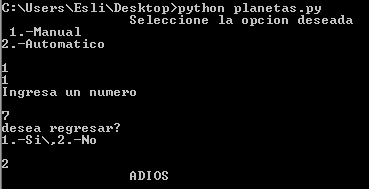
\includegraphics[width=\textwidth, height=7cm]{manual_planetas}
\label{fig:manual_afn}
\caption{Modo manual}
\end{figure}

\begin{figure}[H]
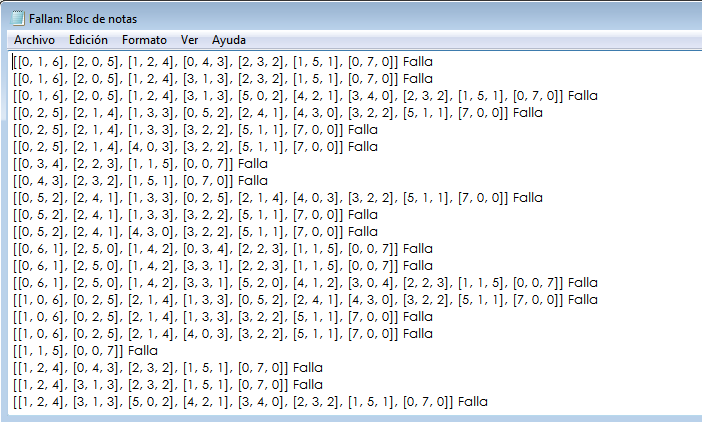
\includegraphics[width=\textwidth, height=7cm]{manual_planetas_salida}
\label{fig:manual_afn}
\caption{Combinaciones que fallan}
\end{figure}
\begin{figure}[H]
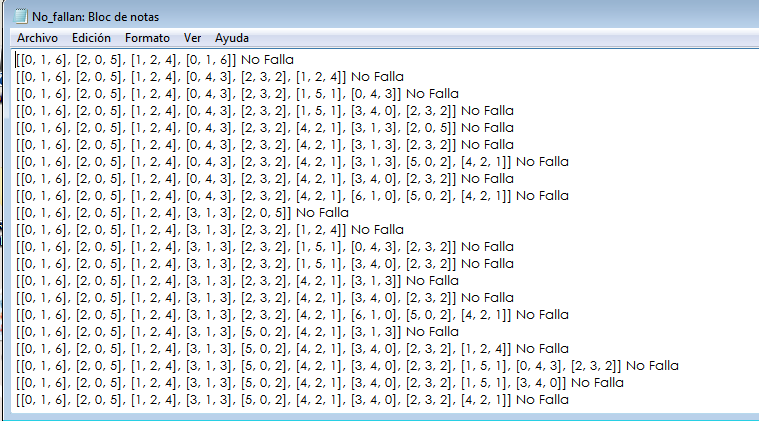
\includegraphics[width=\textwidth, height=7cm]{manual_planetas_salida2}
\label{fig:manual_afn}
\caption{Combinaciones que no fallan}
\end{figure}

\begin{figure}[H]
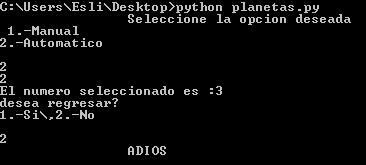
\includegraphics[width=\textwidth, height=7cm]{auto_planetas}
\label{fig:manual_afn}
\caption{Modo Automàtico}
\end{figure}

\begin{figure}[H]
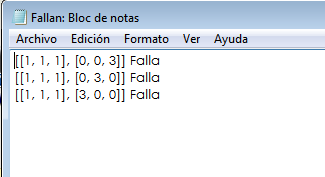
\includegraphics[width=\textwidth, height=7cm]{auto_planetas_salida}
\label{fig:manual_afn}
\caption{Combinaciones que fallan}
\end{figure}
\begin{figure}[H]
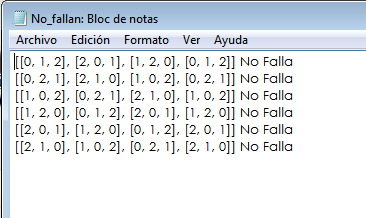
\includegraphics[width=\textwidth, height=7cm]{auto_planetas_salida2}
\label{fig:manual_afn}
\caption{Combinaciones que no fallan}
\end{figure}

\newpage
\section{Palindromo}
Se realizó un programa el cual generara una cadena que sea un palíndromo con una reglas de producción para que genere un palíndromo binario el cual mostrara el, proceso y solo recibirá un dato, en este caso un numero el cual indicara el número de procesos que se llevaran a cabo y la longitud de la cadena.
\subsection{Código fuente}
El programa para está problema fue escrito en el lenguaje Python\\

Archivo: pal.py
\lstset{language=C, breaklines=true, basicstyle=\footnotesize}
\begin{lstlisting}[frame=single]
import random 
def menu():
	entra=1
	fp=open("Palindromo.txt","w")
	fp.close()
	ubi=open ("Camino.txt","w")
	ubi.close()
	while entra==1:
		ubi=open ("Camino.txt","a")
		ubi.close()
		fp=open ("Palindromo.txt","a")
		fp.close()
		print("\n\t\tSeleccione la opcion deseada\n 1.-Manual\n 2.-Automatico\n")
		opc=str(input())
		#opc=str(random.randrange(1,3))
		if opc=='1':
			manual()
		elif opc=='2':
			automatico()
		print("\n\nDesea regresar?\n1.-Si\,2.-No\n")
		entra=int(input())
		#entra=random.randrange(0,2)
	print ("\t\tADIOS\n")
def manual():
	print ("\n\t Usted eligio el modo manual\n Ingrese la longitud del palindromo\n")
	long =int (input ())
	creacion(long)
def automatico():
	print ("\n\t Usted eligio el modo automatico\n ")
	long =int (random.randint(1,1000))
	print (" La longitud del palindromo es: "+str(long))
	creacion(long)
def creacion (long):
	ubi=open ("Camino.txt","a")
	ubi.write('long= '+ str(long)+' --> ')
	derecha=''
	izquierda=''
	palabra=''
	bandera=0
	if (long %2 )!=0:
		repeticiones=int((long-1)/2)
		bandera=1
	else :
		repeticiones=int(long/2)
	for a in range (repeticiones):
		sel=random.randrange(0,2)
		if sel==0:
			derecha='0'+derecha
			izquierda=izquierda+'0'
			ubi.write(' 0 --> ')
		if sel==1:
			derecha='1'+derecha
			izquierda=izquierda+'1'
			ubi.write(' 1 --> ')
	if bandera==1:
		med=random.randrange(0,2)
		if med==0:
			palabra=derecha+'0'+izquierda
			ubi.write(' P --> 0 ')
			ubi.write('\n')
		if med==1:
			palabra=derecha+'1'+izquierda
			ubi.write(' P --> 1 ')
			ubi.write('\n')
	else:
		palabra=derecha+izquierda
		ubi.write(' P --> e ')
		ubi.write('\n')

	primero=derecha+'(P)'+izquierda
	guardar(palabra, primero, long)

def guardar(palabra, primero, long):
	fp=open ("palindromo.txt","a")
	fp.write('long= '+ str(long)+' --> ')
	fp.write(primero+' --> ')
	fp.write(palabra)
	fp.write("\n")
	fp.close()
menu()
\end{lstlisting}

\subsection{Pruebas}
En cuanto a las pruebas, a continuación se mostraran una serie de imágenes capturadas al momento de ejecutar el programa. Los resultados arrojados por el programa anterior son:

\begin{figure}[H]
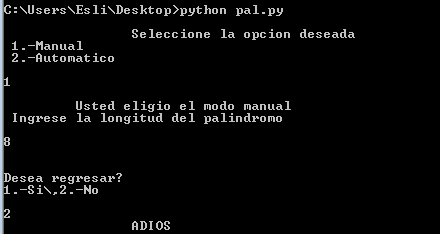
\includegraphics[width=\textwidth, height=7cm]{manual_pal}
\label{fig:manual_afn}
\caption{Modo manual}
\end{figure}

\begin{figure}[H]
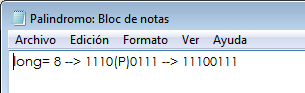
\includegraphics[width=\textwidth, height=7cm]{manual_pal_salida}
\label{fig:manual_afn}
\caption{Salidas}
\end{figure}

\begin{figure}[H]
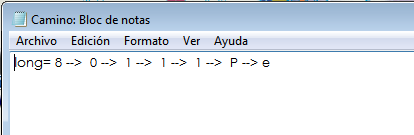
\includegraphics[width=\textwidth, height=7cm]{manual_pal_caminos}
\label{fig:manual_afn}
\caption{Caminos}
\end{figure}

\begin{figure}[H]
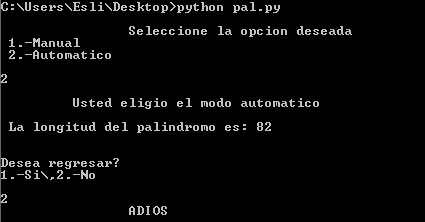
\includegraphics[width=\textwidth, height=7cm]{auto_pal}
\label{fig:manual_afn}
\caption{Modo Automàtico}
\end{figure}

\begin{figure}[H]
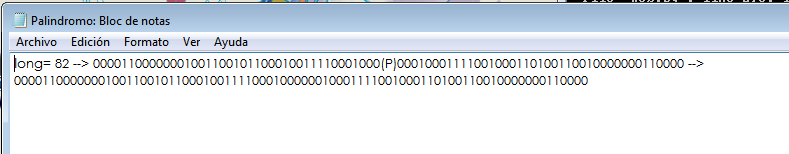
\includegraphics[width=\textwidth, height=7cm]{auto_pal_salida}
\label{fig:manual_afn}
\caption{Salidas}
\end{figure}

\newpage
\section{Paréntesis}
Se realizara la evaluación de una cadena para verificar si la cadena se encuentra balanceada en tanto a los paréntesis haciendo uso de las reglas que tienen la cual entrara en el proceso evaluando la cadena y sustituyendo los caracteres por las reglas dependiendo de los caracteres.
\subsection{Código fuente}
El programa para está problema fue escrito en el lenguaje Python\\

Archivo: paren.py
\lstset{language=C, breaklines=true, basicstyle=\footnotesize}
\begin{lstlisting}[frame=single]

import random 
def manual():
		cadena=""
		ubi=open ("Camino.txt","a")
		ubi.close()
		print ("\t Usted eligio el modo manual\n Ingrese la cadena de parentesis porfavor")
		cadena=input ()
		archivo=open ("Entrada.txt","a")
		archivo.write(cadena)
		archivo.write("\n")
		archivo.close()
		fp=open ("Validado.txt","a")
		fp.close()
		revision(1)
def automatico():
		cadena =""
		ubi=open ("Camino.txt","a")
		ubi.close()
		print ("\t Usted eligio el modo automatico")
		archivo=open ("Automatico.txt","a")
		l=int (random.randrange(5,20))
		print (l)
		cadena=""
		for a in range (l):
			elem=int(random.randrange(0,2))
			if elem==0:
				cadena=cadena+"(" 
			elif elem==1:
				cadena=cadena+")"
		print (cadena)
		archivo.write(cadena)
		archivo.write("\n")
		archivo.close()
		fp=open ("Validado.txt","a")
		fp.close()
		revision(2)
def revision(j):
	if j==1:
		archivo= open("Entrada.txt","r")
	elif j==2:
		archivo= open("Automatico.txt","r")
	y=0
	for linea in archivo:
		cadena=linea
		estados(cadena,y)
		y=y+1
	archivo.close()
def estados(cadena,y):
	ubi=open ("Camino.txt","a")
	caracter=0
	palabra=cadena.split()
	x=0
	ban1=0
	for i in palabra:
		ban1=0
		tamano=len(i)
		#estado=0
		tam=0
		c=0
		nop=0
		lista=['']
		ubi.write(i)
		ubi.write("\n")
		for a in (i+","):	
			if a=='(':
				if c==0 :#veo que sea la primera vez que entre 
					lista.extend('B')
					lista [0]='Inicio'
					print (lista )
					print ("\n")
					ubi.write("".join(lista))
					ubi.write("\n")
					lista.extend ('(RB')
					del lista[1]
					lista [0]='B--> (RB ----->'
					print (lista )
					print ("\n")
					ubi.write("".join(lista))
					ubi.write("\n")
					tam=tam+1
					c=1
				elif c==1:
					if ('R' in lista):
						v=int(lista.index('R')+1)
						lista.insert(v,'R')
						lista.insert(v,'R')
						lista.insert(v,'(')
						lista [0]='R--> (RR ----->'
						del lista [v-1]
						print (lista )
						print ("\n")
						ubi.write("".join(lista))
						ubi.write("\n")
						tam=tam+1
					elif ('B' in lista):
						v=int(lista.index('B')+1)
						lista.insert(v,'B')
						lista.insert(v,'R')
						lista.insert(v,'(')
						lista [0]='B--> (RB ----->'
						del lista [v-1]
						print (lista  )
						print ("\n")
						ubi.write("".join(lista))
						ubi.write("\n")
						tam=tam+1
			elif a==')':
				if ('R' in lista):
					v=int(lista.index('R')+1)
					lista.insert(v,')')
					del lista [v-1]
					lista [0]='R--> ) ----->'
					print (lista )
					print ("\n")
					ubi.write("".join(lista))
					ubi.write("\n")
					tam=tam+1
				else :
					nop==1
					tam=tam+1
			elif a==",":
				if ('B' in lista):
					while ('B ' in lista):
						v=int(lista.index('B')+1)
						lista.insert(v,'')
						del lista [v-1]
						lista [0]='B--> e ----->'
						print (lista )
						print ("\n")
						ubi.write("".join(lista))
						ubi.write("\n")
						tam=tam+1
				if('R' in lista ):
					nop=1
					tam=tam+1
			elif nop==1:
				print ("No valida \n")
				ubi.write(lista)
				ubi.write("no valida \n")
				break
			

		if (('B' in lista) and (tam==len(lista)-2)):
			v=int(lista.index('B')+1)
			lista.insert(v,'')
			del lista [v-1]
			lista [0]='B--> e ----->'
			print (lista )
			print ("\n")
			ubi.write("".join(lista))
			ubi.write("\n")
			guardar (i)
		else:
			print ("------Cadena invalida -------")
			ubi.write("No valida \n")
def guardar(i):
	palabra=i
	valida=open ("Validado.txt","a")
	valida.write(palabra)
	valida.write(" \n")
	valida.close()
def menu():
	entra=1
	fp=open ("Validado.txt","w")
	fp.close()
	ubi=open ("Camino.txt","w")
	ubi.close()
	archivo=open ("Automatico.txt","w")
	archivo1=open ("Entrada.txt","w")
	while entra==1:
		print("\t\tSeleccione la opcion deseada\n 1.-Manual\n2.-Automatico\n")
		opc=str(input())
		#opc=str(random.randrange(1,3))
		print(opc)
		if opc=='1':
			manual()
		elif opc=='2':
			automatico()
		print("desea regresar?\n1.-Si\,2.-No\n")
		entra=int(input())
		#entra=random.randrange(0,2)
	print ("\t\tADIOS\n")

menu()

\end{lstlisting}

\subsection{Pruebas}
En cuanto a las pruebas, a continuación se mostraran una serie de imágenes capturadas al momento de ejecutar el programa. Los resultados arrojados por el programa anterior son:

\begin{figure}[H]
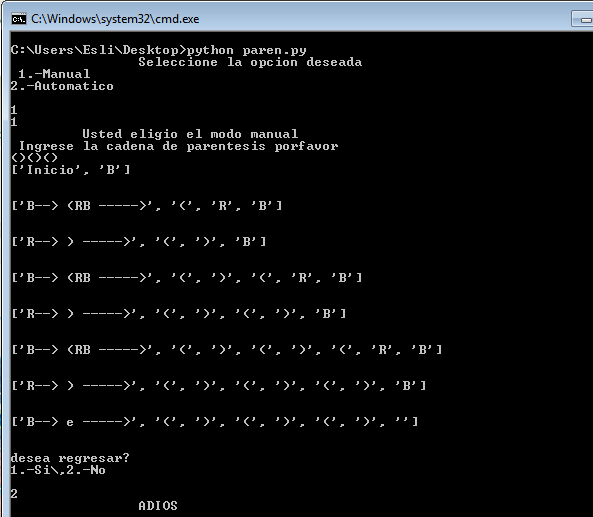
\includegraphics[width=\textwidth, height=10cm]{manual_paren}
\label{fig:manual_afn}
\caption{Modo Manual}
\end{figure}

\begin{figure}[H]
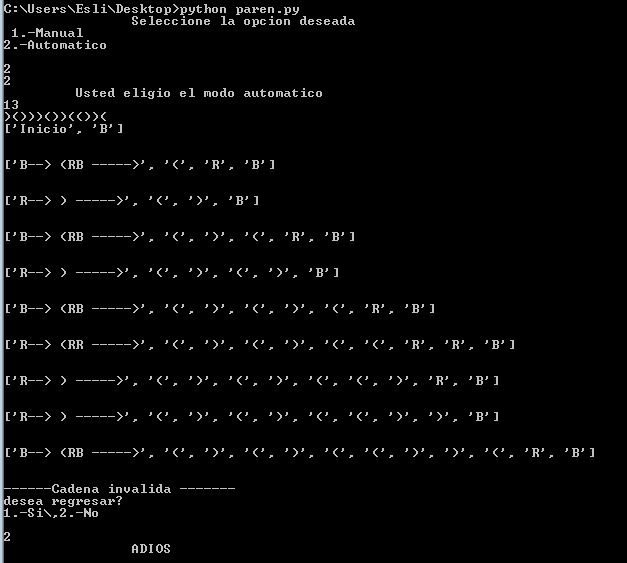
\includegraphics[width=\textwidth, height=15cm]{auto_paren}
\label{fig:manual_afn}
\caption{Modo Automatico}
\end{figure}

\newpage
\section{Pila}
El programa hace uso de la estructura ‘Pila’ ya que su autómata realiza ese proceso, al realizarlo en Python se forma la clase con funciones que caracterizan a una pila con un pop y push. El programa consiste con una cadena de 0’s y 1’s la cual evaluara que cada que entra un cero meta una X en la pila y al momento de que entra un 1 lo saca. Al final evalúa si la pila esta vacía y con esto verifica si la cadena esta balanceada en cuanto a su número de 0’s y 1’s.
\subsection{Código fuente}
El programa para está problema fue escrito en el lenguaje Python\\

Archivo: claspila.py
\lstset{language=C, breaklines=true, basicstyle=\footnotesize}
\begin{lstlisting}[frame=single]

class Pila:
	lista=[]
	tope=0
	def inicializar(self):
		self.lista=[]
		self.lista.append('Z0')
		self.tope=self.tope+1

	def push (self):
		self.lista.insert(self.tope-1, 'X')
		self.tope= self.tope+1

	def pop (self):
		del self.lista[0]
		self.tope=self.tope-1

\end{lstlisting}

Archivo: pila.py
\lstset{language=C, breaklines=true, basicstyle=\footnotesize}
\begin{lstlisting}[frame=single]
import claspila
import random
from time import *
from tkinter import *
def menu():
	entra=1
	fp=open ("Validado.txt","w")
	fp.close()
	fp1=open ("Camino.txt","w")
	while entra==1:
		print("\t\tSeleccione la opcion deseada\n 1.-Manual\n2.-Automatico\n")
		opc=str(input())
		#opc=str(random.randrange(1,3))
		print(opc)
		if opc=='1':
			manual()
		elif opc=='2':
			automatico()
		print("desea regresar?\n1.-Si\,2.-No\n")
		entra=int(input())
		#entra=random.randrange(0,2)
	print ("\t\tADIOS\n")
def manual():
		archivo1=open ("Entrada.txt","w")
		cadena=""
		ubi=open ("Camino.txt","a")
		ubi.close()
		print ("\t Usted eligio el modo manual\n Ingrese la cadena de 0's y 1's porfavor")
		cadena=input ()
		archivo=open ("Entrada.txt","a")
		archivo.write(cadena)
		archivo.write("\n")
		archivo.close()
		revision(1)
def automatico():
	archivo=open ("Automatico.txt","w")
	cadena =""
	ubi=open ("Camino.txt","a")
	ubi.close()
	print ("\t Usted eligio el modo automatico")
	archivo=open ("Automatico.txt","a")
	l=int (random.randrange(5,20))
	print (l)
	cadena=""
	for a in range (l):
		elem=int(random.randrange(0,2))
		if elem==0:
			cadena=cadena+"1" 
		elif elem==1:
			cadena=cadena+"0"
	print (cadena)
	archivo.write(cadena)
	archivo.write("\n")
	archivo.close()
	revision(2)
def revision(j):
	if j==1:
		archivo= open("Entrada.txt","r")
	elif j==2:
		archivo= open("Automatico.txt","r")
	y=0
	for linea in archivo:
		cadena=linea
		estados(cadena,y)
		y=y+1
	archivo.close()
def eliminar(cadena):
	x=1
	cad=""
	while(x<len(cadena)):
		cad+=cadena[x]
		x+=1
	return cad
def estados(cadena,y):
	root = 	Tk()
	canvas=Canvas(root,width=450,height=450)
	canvas.pack()
	ubi=open ("Camino.txt","a")
	caracter=0
	palabra=cadena.split()
	x=0
	for i in palabra:
		eliminacion=palabra[0]
		ban=0
		pila=claspila.Pila()
		pila.inicializar()
		cad="".join(pila.lista)
		print('Inicio |-' +cad) 
		print ('\n')
		ubi.write("------"+i+"------\n")
		ubi.write("Inicio  |-")
		ubi.write("".join(pila.lista))
		ubi.write("\n")
		canvas.create_line(175,150,175,50)
		canvas.create_line(175,300,175,400)
		estado=Label(root,text="                                                                      ",font=("Arial",12))
		estado.place(x = 170, y = 35)
		estado=Label(root,text=eliminacion,font=("Arial",12))
		estado.place(x = 170, y = 35)
		estado=Label(root,text="                                                                      ",font=("Arial",12))
		estado.place(x = 170, y = 400)
		estado=Label(root,text=str(pila.lista),font=("Arial",12))
		estado.place(x = 170, y = 400)
		estado=Label(root,text=" p "+"  ",font=("Arial",50),fg="black")
		estado.place(x = 150, y = 180)
		sleep(1)
		root.update()
		for a in (i+","):	
			if a=='0':
				pila.push()
				canvas.create_line(175,150,175,50)
				canvas.create_line(175,300,175,400)
				estado=Label(root,text="                                                                      ",font=("Arial",12))
				estado.place(x = 170, y = 35)
				print(eliminacion)
				eliminacion=eliminar(eliminacion)
				print(eliminacion)
				estado=Label(root,text=eliminacion,font=("Arial",12))
				estado.place(x = 170, y = 35)
				estado=Label(root,text="                                                                      ",font=("Arial",12))
				estado.place(x = 170, y = 400)
				estado=Label(root,text=str(pila.lista),font=("Arial",12))
				estado.place(x = 170, y = 400)
				estado=Label(root,text=" p "+"  ",font=("Arial",50),fg="black")
				estado.place(x = 150, y = 180)
				sleep(1)
				root.update()
				cad="".join(pila.lista)
				print ('|-'+cad)
				print ('\n')
				ubi.write("|-")
				ubi.write("".join(pila.lista))
				ubi.write("\n")
			elif a=='1' and pila.tope>1:
				pila.pop()
				canvas.create_line(175,150,175,50)
				canvas.create_line(175,300,175,400)
				estado=Label(root,text="                                                                      ",font=("Arial",12))
				estado.place(x = 170, y = 35)
				eliminacion=eliminar(eliminacion)
				estado=Label(root,text=eliminacion,font=("Arial",12))
				estado.place(x = 170, y = 35)
				estado=Label(root,text="                                                                      ",font=("Arial",12))
				estado.place(x = 170, y = 400)
				estado=Label(root,text=str(pila.lista),font=("Arial",12))
				estado.place(x = 170, y = 400)
				estado=Label(root,text=" q "+"  ",font=("Arial",50),fg="black")
				estado.place(x = 150, y = 180)
				sleep(1)
				root.update()
				cad="".join(pila.lista)
				print ('|-'+cad)
				print ('\n')
				ubi.write("|-")
				ubi.write("".join(pila.lista))
				ubi.write("\n")
			elif a==',' and pila.lista[0]=='Z0' and ban==0:
				print ("---Cadena Valida---")
				ubi.write("---Cadena Valida------------\n")
				guardar(i)
				canvas.create_line(175,150,175,50)
				canvas.create_line(175,300,175,400)
				estado=Label(root,text="                                                                      ",font=("Arial",12))
				estado.place(x = 170, y = 35)
				eliminacion=eliminar(eliminacion)
				estado=Label(root,text=eliminacion,font=("Arial",12))
				estado.place(x = 170, y = 35)
				estado=Label(root,text="                                                                      ",font=("Arial",12))
				estado.place(x = 170, y = 400)
				estado=Label(root,text=str(pila.lista),font=("Arial",12))
				estado.place(x = 170, y = 400)
				estado=Label(root,text=" f "+"  ",font=("Arial",50),fg="black")
				estado.place(x = 150, y = 180)
				sleep(1)
				root.update()
			else:
				ban=1
				print ("---Cadena NO Valida---")
				ubi.write("----Cadena NO Valida----\n")
	root.mainloop()

def guardar(i):
	valida=open ("Validado.txt","a")
	valida.write(i)
	valida.write(" \n")
	valida.close()
menu()

\end{lstlisting}

\subsection{Pruebas}
En cuanto a las pruebas, a continuación se mostraran una serie de imágenes capturadas al momento de ejecutar el programa. Los resultados arrojados por el programa anterior son:


\begin{figure}[H]
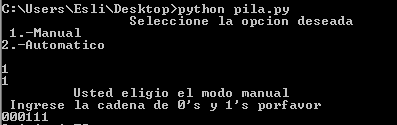
\includegraphics[width=\textwidth, height=7cm]{manual_pila}
\label{fig:manual_afn}
\caption{Modo Manual}
\end{figure}

\begin{figure}[H]
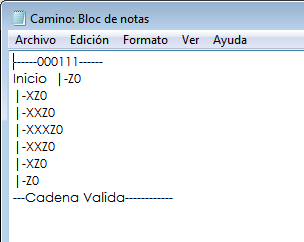
\includegraphics[width=\textwidth, height=7cm]{manual_pila_caminos}
\label{fig:manual_afn}
\caption{Caminos}
\end{figure}

\begin{figure}[H]
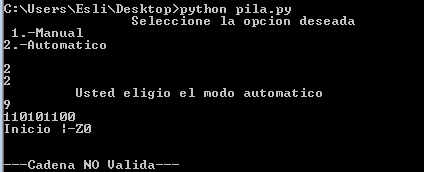
\includegraphics[width=\textwidth, height=7cm]{auto_pila}
\label{fig:manual_afn}
\caption{Modo Automàtico}
\end{figure}

\begin{figure}[H]
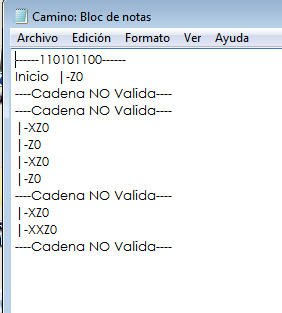
\includegraphics[width=\textwidth, height=10cm]{auto_pila_caminos}
\label{fig:manual_afn}
\caption{Caminos}
\end{figure}

\begin{figure}[H]
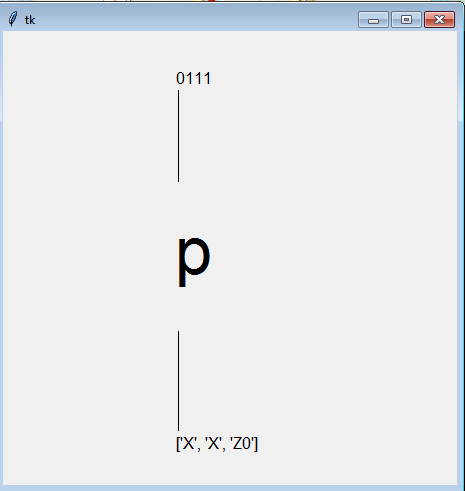
\includegraphics[width=\textwidth, height=14cm]{pila_grafico}
\label{fig:manual_afn}
\caption{Grafico}
\end{figure}

\newpage
\section{Máquina de Turing}
La máquina de Turing que se empleo fue para que revisara si una cadena que está compuesta de 0’s y 1’s verifica si primero están los ceros y luego los unos conforme a la relación de 0n 1n en caso de que sea así, la cadena va sustituyendo los 0’s por X y los 1’s por Y así hasta que localiza una B.
\subsection{Código fuente}
El programa para está problema fue escrito en el lenguaje Python\\

Archivo: maquina.py
\lstset{language=C, breaklines=true, basicstyle=\footnotesize}
\begin{lstlisting}[frame=single]
import random
def menu():
	entra=1
	fp=open ("Validado.txt","w")
	fp.close()
	fp1=open ("Camino.txt","w")
	while entra==1:
		print("\t\tSeleccione la opcion deseada\n 1.-Manual\n2.-Automatico\n")
		opc=str(input())
		#opc=str(random.randrange(1,3))
		print(opc)
		if opc=='1':
			manual()
		elif opc=='2':
			automatico()
		print("desea regresar?\n1.-Si\,2.-No\n")
		entra=int(input())
		#entra=random.randrange(0,2)
	print ("\t\tADIOS\n")
def manual():
		archivo1=open ("Entrada.txt","w")
		cadena=""
		ubi=open ("Camino.txt","a")
		ubi.close()
		print ("\t Usted eligio el modo manual\n Ingrese la cadena de 0's y 1's porfavor")
		cadena=input ()
		archivo=open ("Entrada.txt","a")
		archivo.write(cadena)
		archivo.write("\n")
		archivo.close()
		revision(1)
def automatico():
	archivo=open ("Automatico.txt","w")
	cadena =""
	ubi=open ("Camino.txt","a")
	ubi.close()
	print ("\t Usted eligio el modo automatico")
	archivo=open ("Automatico.txt","a")
	l=int (random.randrange(5,1000))
	print (l)
	cadena=""
	for a in range (l):
		elem=int(random.randrange(0,2))
		if elem==0:
			cadena=cadena+"1" 
		elif elem==1:
			cadena=cadena+"0"
	print (cadena)
	archivo.write(cadena)
	archivo.write("\n")
	archivo.close()
	revision(2)
def revision(j):
	if j==1:
		archivo= open("Entrada.txt","r")
	elif j==2:
		archivo= open("Automatico.txt","r")
	for linea in archivo:
		cadena=linea
		estados(cadena)
	archivo.close()
def estados(cadena):
	ubi=open ("Camino.txt","a")
	caracter=0
	palabra=cadena.split()
	palabra=palabra
	x=0
	for i in (palabra):
		v=i+"B"
		ban=0
		lista=[]
		index=0
		ubi=open ("Camino.txt","a")
		lista.extend(v)
		lista.insert(index,'---- Inicio -----> ')
		proceso (lista)
		del lista[index]
		cad=" ".join(lista)
		lista.insert(index,' q0->')
		proceso (lista)
		del lista [index]
		estado=0
		sigue=1
		while sigue==1:
			if estado==0:
				if lista[index]=='0':	
					lista.insert(index+1,' q1->')
					lista[index]="X"
					proceso(lista)
					del lista[index+1]
					index =index+1
					estado=1
				elif lista[index]=='Y':
					lista.insert(index+1,' q3->')
					lista[index]="Y"
					proceso(lista)
					del lista[index+1]
					index=index+1
					estado=3
				else :
					sigue=0
					lis=[]
					lis.extend('No Valida')
					proceso(lis)
			elif estado==1:
				if lista[index]=='0':	
					lista.insert(index+1,' q1->')
					lista[index]="0"
					proceso(lista)
					del lista[index+1]
					index =index+1
					estado=1
				elif lista[index]=='1':
					lista[index]="Y"
					lista.insert(index-1,' q2->')
					proceso(lista)
					del lista[index-1]
					index=index-1
					estado=2
				elif lista[index]=='Y':
					lista.insert(index+1,' q3->')
					lista[index]="Y"
					proceso(lista)
					del lista[index+1]
					index=index+1
					estado=1
				else :
					sigue=0
					lis=[]
					lis.extend('No Valida')
					proceso(lis)
			elif estado==2:
				if lista[index]=='0':
					lista[index]="0"	
					lista.insert(index-1,' q1->')
					proceso(lista)
					del lista[index-1]
					index =index-1
					estado=2
				elif lista[index]=='X':
					lista[index]="X"
					lista.insert(index+1,' q0->')
					proceso(lista)
					del lista[index+1]
					index=index+1
					estado=0
				elif lista[index]=='Y':
					lista[index]="Y"
					lista.insert(index-1,' q3->')
					proceso(lista)
					del lista[index-1]
					index=index-1
					estado=2
				else :
					sigue=0
					lis=[]
					lis.extend('No Valida')
					proceso(lis)
			if estado==3:
				if lista[index]=='B':	
					lista[index]="B"
					lista.insert(index-1,' q4-> ')
					proceso(lista)
					del lista[index-1]
					lista.insert (index+1, '------Fin Valida------')
					proceso (lista)
					index =index+1
					estado=4
					guardar(i)
					sigue=0
				elif lista[index]=='Y':
					lista.insert(index+1,' q4->')
					lista[index]="Y"
					proceso(lista)
					del lista[index+1]
					index=index+1
					estado=3
				else :
					sigue=0
					lis=[]
					lis.extend('No Valida')
					proceso(lis)


def proceso(lista):
	ubi=open ("Camino.txt","a")
	cad=" ".join(lista)
	print ('|-  '+cad)
	print ('\n')
	ubi.write("|-  ")
	ubi.write(" ".join(lista))
	ubi.write("\n")

def guardar(i):
	valida=open ("Validado.txt","a")
	valida.write(i)
	valida.write(" \n")
	valida.close()
menu()
\end{lstlisting}

\subsection{Pruebas}
En cuanto a las pruebas, a continuación se mostraran una serie de imágenes capturadas al momento de ejecutar el programa. Los resultados arrojados por el programa anterior son:

\begin{figure}[H]
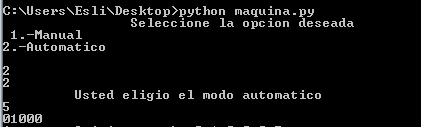
\includegraphics[width=\textwidth, height=7cm]{auto_maquina}
\label{fig:manual_afn}
\caption{Modo Automàtico}
\end{figure}

\begin{figure}[H]
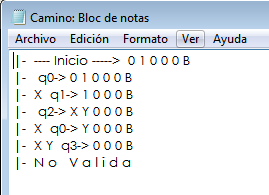
\includegraphics[width=\textwidth, height=7cm]{auto_maquina_camino}
\label{fig:manual_afn}
\caption{Caminos}
\end{figure}

\begin{figure}[H]
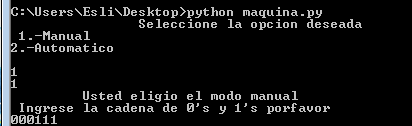
\includegraphics[width=\textwidth, height=7cm]{manual_maquina}
\label{fig:manual_afn}
\caption{Modo Manual}
\end{figure}

\begin{figure}[H]
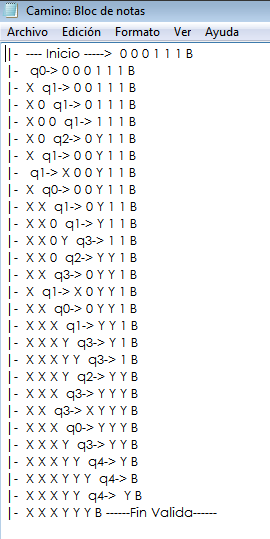
\includegraphics[width=\textwidth, height=20cm]{manual_maquina_caminos}
\label{fig:manual_afn}
\caption{Caminos}
\end{figure}

\begin{figure}[H]
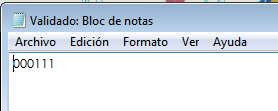
\includegraphics[width=\textwidth, height=7cm]{manual_maquina_validos}
\label{fig:manual_afn}
\caption{Validos}
\end{figure}
\end{document}